\section{Force calculations | tree algorithms and particle mesh technique}
\thispagestyle{plain}

We have discretized our N-body system using fiducial macro-particles.
The equations of motion are given by
\begin{equation}
    \vec{\ddot{x}}=-\vec{\nabla} \phi\left(\vec{x}_i\right), \quad \phi(\vec{x})=-G \sum_{j=1}^N \frac{m_j}{\left[\left(\vec{x}-\vec{x}_j\right)^2+\epsilon^2\right]^{\frac{1}{2}}}
\end{equation}
\bluebox{\textbf{Integration in time: }Given the forces on the particles, we can integrate this ordinary
differential equation in time. Classically a symplectic method like leapfrog would be used. But
modern N-body-packages like Rebound use high-order adaptive-step-size integrators. See section \ref{sec:symplectic_integrators} for details.}

But how can we calculate the forces on the particles given the particle positions?

\subsection{Calculating the forces | Direct summation}
We can simply and exactly calculate

\begin{equation}
    \vec{\ddot{x}}_i=-G \sum_{j=1}^N \frac{m_j}{\left[\left(\vec{x}_i-\vec{x}_j\right)^2+\epsilon^2\right]^{\frac{3}{2}}}\left(\vec{x}_i-\vec{x}_j\right)
\end{equation}

\problem{For the force on each of the $N$ particles, $N-1$ terms have to be evaluated and summed - so in total we have $\mathcal{O}(N^2)$ operations. For $t_\text{relax}$ to be large (so the simulated time can be large), $N$ must be large. But even for $N = 10^{10}$ assuming we can to $N = 10^6$ in one month of computer time, we'd need to run our computer $\sim 10^7$ years.}

\subsection{Overview on faster, approximate force calculation schemes}
\begin{itemize}
    \item \textbf{tree algorithms} - distant groups do not need to be resolved in every detail to calculate their respective forces - some or even one term of the multipole expansion can be used. Generally we can construct hierarchical multipole methods where a tree is a method to partition space based on the particle distribution.
    \item \textbf{particle mesh methods} - from the particle distribution, a mass density on a grid is calculated and using
    \begin{itemize}
        \item \textbf{fourier transform based methods} to calculate the potential from the Poisson equation and the density distribution (the necessary convolution is a multiplication in Fourier space and FFT is fast ($\mathcal{O}(N \log N)$))
        \item \textbf{iterative solvers} relaxation methods to solve the Poisson equation
    \end{itemize}
    the forces on gridpoints can be calculated and interpolated to the particles.
\end{itemize}

We can often combine the different force calculation approaches and use direct 
summation on small scales. To speed things up we use GPUs that are very fast for 
easy parallel operations like (block) matrix multiplication.

\subsection{Faster method I | Multipole expansion | tree algorithms}
\idea{In tree algorithms the force on one particle is calculated based on multipole expansions
of groups in the \textit{far-field} rather than individual particles (see figure \ref{fig:multipole}),
while the \textit{near-field} is calculated exactly.}

Consider the simple example where we want to calculate the force (and with this the
movement) of a single particle based on the interaction with a distant group of particles.
If the group spans only a small angle of the particles view-field, the force acting
on the particle can be approximated by the one along the axis to the groups center of mass, so

\begin{equation}
    \begin{gathered}
        \vec{a}_\text{our particle} \approx -GM \frac{\vec{r}_\text{our particle} - \vec{s}}{||\vec{r}_\text{our particle} - \vec{s}||^3} \\ \quad \text{group's mass } M, \quad \text{ group's center of mass } \vec{s}
    \end{gathered}
\end{equation}

Further details of the group can be resolved by higher order terms of the multipole expansion.

In the following we need to answer
\begin{itemize}
    \item How do we resolve the potential of a group in less detail? (the simple monopole term in the force above will often be enough) When will this be accurate?
    \item How can derive a scheme, so that for the force on each particle, not all others have to be considered, but groups under small opening angle are only resolved as a whole (e.g. by the monopole term)?
\end{itemize}

\begin{figure}[H]
    \centering
    \includesvg[width=0.8\textwidth]{figures/multipole.svg}
    \caption{If the opening angle of a group is small enough, the force can be approximated by the monopole term at its center of mass.}
    \label{fig:multipole}
\end{figure}

The exact potential of the group measured at $\vec{r}$ is

\begin{equation}
    \phi(\vec{r})=-G \sum_i \frac{m_i}{\left\|\vec{r}-\vec{x}_i\right\|}
\end{equation}

\subsubsection{Deriving the multipole expansion}
Let us rewrite the potential of the group as
\begin{equation}
    \phi(\vec{r})=-G \sum_i \frac{m_i}{\left\|\vec{r}-\vec{s}+\vec{s}-\vec{x}_i\right\|}, \quad \text { group center of mass } \vec{s}=\frac{1}{M} \sum_i m_i \vec{x}_i
\end{equation}
and define $\vec{y} := \vec{r} - \vec{s}$ and $\vec{l} = \vec{s} - \vec{x}_i$.
We Taylor expand with respect to $\vec{l}$ around $\vec{l} = 0$.

\bluebox{\textbf{Multivariate Taylor expansion: }
    \begin{equation}
        f(\vec{x}+\vec{h}) = f(\vec{x}) + \vec{h} \cdot \vec{\nabla} f(\vec{x}) + \frac{1}{2} \vec{h}^T \left. \mat{H}_f \right|_\vec{x} \vec{h} + \mathcal{O}(\vec{h}^3)
    \end{equation}
    where $\mat{H}_f$ is the Hessian matrix of $f$, the Jacobian of the gradient of $f$.}
with this we get
\begin{equation}
    f(\vec{y}+\vec{l})=\frac{1}{\left\|\vec{y}+\vec{s}-\vec{x}_i\right\|}=\frac{1}{\|\vec{y}\|}+\frac{\vec{y} \cdot \vec{l}}{\|\vec{y}\|^3}+\frac{1}{2} \underbrace{\frac{\vec{l}^T\left[3 \vec{y} \vec{y}^T-\vec{y}^2 1\right] \vec{l}}{\|\vec{y}\|^5}}_{=\frac{\vec{y}^T\left[3 \vec{l} \vec{l}^T-\vec{l}^2 1\right] \vec{y}}{\|\vec{y}\|^5}}+\cdots
\end{equation}
The numerators summed over all particles in the group lead to the \textit{moments}
\begin{equation}
    \begin{aligned}
    & \text { monopole: } M=\sum_i m_i, \quad \text { dipole }: \vec{D}=\sum_i m_i\left(\vec{s}-\vec{x}_i\right), \\
    & \text { quadrupole: } Q_{i j}=\sum_k m_k\left[3\left(\vec{s}-\vec{x}_i\right)\left(\vec{s}-\vec{x}_i\right)^T-\left(\vec{s}-\vec{x}_i\right)^2 \delta_{i j}\right]
    \end{aligned}
\end{equation}

\note{The gravitational dipole moment (asymmetry of the mass distribution around the center of mass) vanishes as of the definition of the center of mass.}

\subsubsection{Multipole expansion}
Up to the quadrupole term, the potential of the group can be written as
\begin{equation}
    \phi(\vec{r})=-G\left(\frac{M}{\|\vec{y}\|}+\frac{1}{2} \frac{\vec{y}^{T} \mat{Q} \vec{y}}{\|\vec{y}\|^5}\right), \quad \vec{y}=\vec{r}-\vec{s}, \quad \text { center of mass } \vec{s}
\end{equation}
which we expect to be accurate if
\begin{equation}
    \theta \underset{\text{small angle}}{\approx} \frac{\langle ||\vec{x}_i - \vec{s}|| \rangle}{||\vec{y}||} \approx \frac{l}{y} \ll 1, \quad \text{radius } l \text{ of the group}
\end{equation}
so in other words if the distance
of our point of interest to the center of mass
of the group $\vec{y} = \vec{r} - \vec{s}$ is much 
larger than the radius of the group $l$.

\subsubsection{Hierarchical grouping | baseline for smart force calculations}
Let us split the particles into hierarchical groups (so a tree structure
with groups and subgroups ...), which will later allow
us to resolve details in the force on a particle as necessary. For all groups
we calculate the multipole moments we want to consider (e.g. only the monopole, i.e.
the total mass) and the center of mass.

\subsubsubsection{Cosntructing the tree | Barnes and Hut oct-tree}
The Barnes and Hut algorithm goes as
\begin{enumerate}
    \item start with a cube containing all particles
    \item subdivide the cube into 8 sub-cubes
    \item if a cube contains more than one particle, to back to step 2 (recursion)
    \item Empty sub-cubes are not stored
\end{enumerate}
we therefore grow a tree with particles as leaves to purity.

In 2D we have a quad-tree (illustrated in figure \ref{fig:quad_tree}), in 1D a binary tree.

\begin{figure}[H]
    \centering
    \includesvg[width=0.8\textwidth]{figures/quad_tree.svg}
    \caption{The Barnes and Hut algorithm constructs a tree with particles as leaves.}
    \label{fig:quad_tree}
\end{figure}

\begin{itemize}
    \item \textcolor{green1}{Advantage - auto-adaptation}: There is more refinement in dense areas and less in less dense areas.
    \item \textcolor{red1}{Disadvantage - things can go deep}: The deepest level depends on the smallest separation of two particles - things go very deep if two particles are very close to each other and do not naturally fall onto some border.
\end{itemize}

\paragraph*{Tree construction and calculation of the multipole moments}
\begin{enumerate}
    \item Build the tree by sequentially adding particles. Splits into sub-nodes are done, until the particle can be placed inside an empty sub-node.
    \item Recursively compute the multipole moments
    \begin{itemize}
        \item Does the node have sub-nodes?
        \begin{itemize}
            \item \textbf{Yes:} Compute the multipole moments of the sub-nodes, then calculate the node's-moments based on them. For the monopole, we just have to sum the masses of the subnodes go get the monopole moment, the center of mass is the weighted average of the subnodes' centers of mass.
            \item \textbf{No:} The moments should be trivial (monopole: just the particle mass, center of mass is the particle position).
        \end{itemize}
    \end{itemize}
\end{enumerate}

\paragraph*{Alternative grouping to the Barnes and Hut algorithm - kd-trees}
Alternatively, binary subdivisions along the axis can be done to do splits
as illustrated in figure \ref{fig:kd_tree}. The splitting can
e.g. be done to balance fraction of mass. \textcolor{green1}{Advantage}: The depth
of the tree can easily be controlled; \textcolor{red1}{disadvantage}: 
we have to store all the splitting planes - complicated bookkeeping.

\begin{figure}[H]
    \centering
    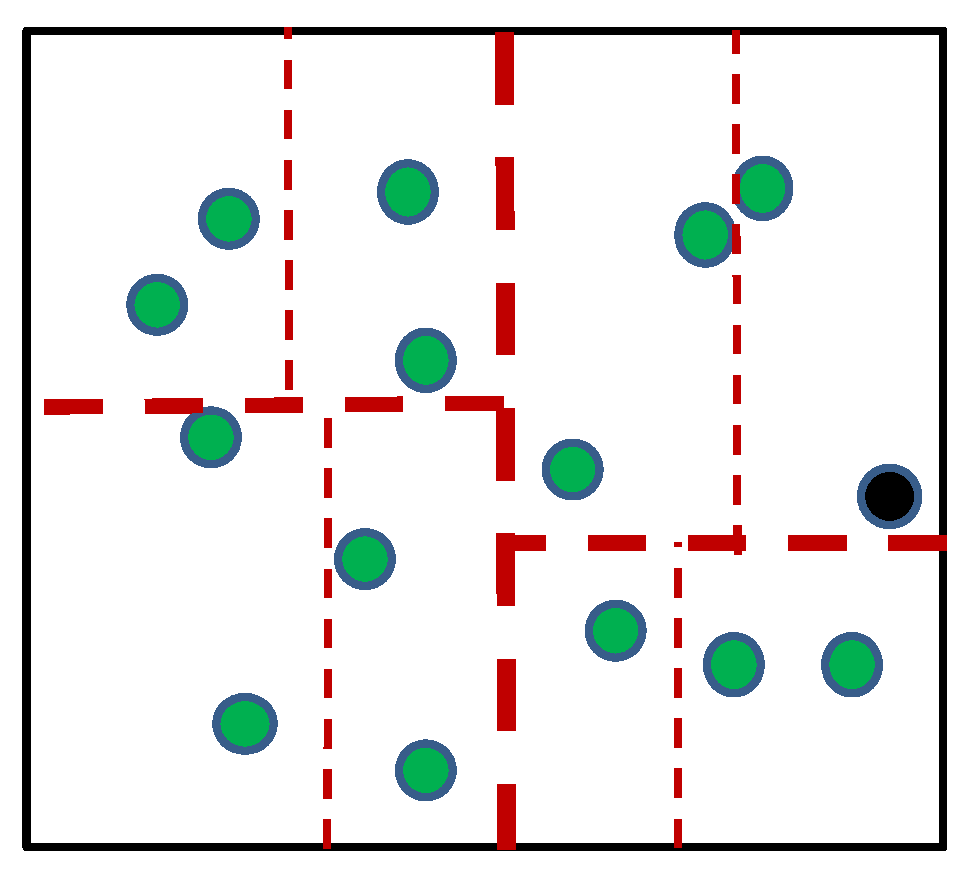
\includegraphics[width=0.4\textwidth]{figures/kd_tree.pdf}
    \caption{The kd-tree - binary subdivisions along the axes.}
    \label{fig:kd_tree}
\end{figure}

\subsubsection{Tree walk - force calculation with adaptive group resolution}
We want to calculate the force on each of our $N$ particles, without
considering all $N-1$ other particles (in total $\mathcal{O}(N^2)$ operations).
\greenbox{Based on the hierarchical grouping and 
calculated multipole moments, we can reach $\mathcal{O}(N \log N)$ (derivation follows). The idea
is to for each particle calculate an approximate force acting on it using the
tree-walk algorithm.}
\subsubsubsection{Tree walk algorithm}
For each of the $N$ particles, to calculate the force we
starting at the root of the tree check for the opening angles of
the sub-groups, as illustrated in figure \ref{fig:tree_walk}.

\begin{figure}[H]
    \centering
    \includesvg[width=0.8\textwidth]{figures/tree_walk.svg}
    \caption{When do we walk further down the tree?}
    \label{fig:tree_walk}
\end{figure}

For each node consider the opening angle $\theta$
\begin{itemize}
    \item $\theta < \theta_c$ (smaller than critical angle): calculate the force from this node at our point of interest based on the multipole (or simply monopole) expansion. This is added to the total force at the point of interest.
    \item $\theta > \theta_c$ (larger than critical angle): open the subnodes of this node recurse
\end{itemize}

\greenbox{\textbf{Error control by $\theta_c$: } The smaller $\theta_c$ the more expensive but also exact the force calculation. For $\theta_c = 0$ we are back at direct summation.}

\paragraph*{Fast multipole methods} In our current method we calculate an approximate force for each of our $N$ particles and then forward them based on this. In a further approximation, we can use, that the potential of a distant group feld by nearby particles will be similar - this 
is cheaper but also harder to parallelize.

\subsubsubsection{Derivation of the cost of the tree based force calculation | $\mathcal{O}(N \log N)$}
Consider $N$ homogeneously distributed particles in a sphere with radius $R$.
Now consider a particle at the center of the sphere. At a distance $r$ from
it, the node-size which we have so resolve in the force calculation can be estimated as
\begin{equation}
    l^3(r), \quad l(r) \approx \theta_c r
\end{equation}
So taking the mean particle distance
\begin{equation}
    d=\left[\frac{\left(\frac{4 \pi}{3}\right) R^3}{N}\right]^{1 / 3}
\end{equation}
as the minimum distante at which other particles have to be considered, we can estimate
\begin{equation}
    \begin{gathered}
        \# \text{ nodes to be considered in the force calculation} \\ \text{ for one particle } \approx \int_d^R \frac{4 \pi r^2 d r}{l^3(r)}=\frac{4 \pi}{\theta_c^3} \ln \frac{R}{d} \propto \frac{\ln N}{\theta_c^3}
    \end{gathered}
\end{equation}

\bluebox{As we have $N$ particles with $\sim \log N$ interactions each, the total cost of the force calculation is $\mathcal{O}(N \log N)$, much
better than the $\mathcal{O}(N^2)$ of direct summation.}

\subsubsubsection{Expected typical force errors in a monopole approximation | $(\Delta F_{\text{tot}}) \propto \theta_c^7$}
We estimate the force error when resolving a group only based on the monopole
(so as if all mass was concentrated at the center of mass) by the difference
to the situation where all mass would be concentrated at the groups edge
(group radius $l$).
\begin{equation}
    \Delta F_{\text {node }} \sim\left|F_c-F_x\right|=\left|\frac{G M_{\text {node }}}{r^2}-\frac{G M_{\text {node }}}{r^2+l^2}\right| \underset{\frac{1}{1+x} \approx 1-x \\ x \ll 1}{\approx} \frac{G M_{\text {node }}}{r^2} \frac{l^2}{r^2}=\frac{G M_{\text {node }}}{r^2} \theta_c^2
\end{equation}
plugging in $M_\text{node} = \frac{M}{N_\text{nodes}}$ with $N_\text{nodes} \propto \theta^3_c$ (as previously found),
and summing over all nodes (akin to how variance adds up in the random walk), we get

\begin{equation}
    \begin{gathered}
        \text{total squared error in the force calculation for one particle based on monopole approximations: }\\
        \Delta F_{\text{tot}} \sim N_{\text{nodes}} \Delta F_{\text{node}} \propto \theta_c^7 \rightarrow |F_{\text{tot}}| \propto \theta_c^{3.5}
    \end{gathered}
\end{equation}

so \textcolor{blue1}{roughly inversely proportional to the computational cost for this particle} (as $N_{\text{nodes}} \propto \theta_c^{-3}$).

\yellowbox{The smaller the opening angle, the higher the cost, the smaller the error.}

\subsection{Faster method II | Particle mesh technique for efficiently computing long-ranged forces}
Consider for instance a plasma. Coulomb interactions are short-ranged,
occuring on the scale of the Debye length (as of the shielding
effect of charge) while gravity is long-ranged.
\problem{Direct summation is $\mathcal{O}(N^2)$ and all interactions are considered. However, for the short ranged
interactions of a particle, only a few others in the vicinity are important and the long range interactions
can safely be approximated.}
\idea{Split the potential into one part describing short-ranged interactions and one part describing long-ranged interactions.
\begin{equation}
    V = V^{\text{short}} + V^{\text{long}}
\end{equation}
Calculate $V^{\text{short}}$ using direct summation and $V^{\text{long}}$ using the \textbf{particle mesh technique}.}

\greenbox{The central idea of the particle mesh method is to use an auxiliary mesh on which the potential can be quickly calculated based on the methods discussed for the Poisson equation (multigrid relaxation or Fourier techniques).}

\subsubsection{Schematic particle mesh algorithm}
\begin{enumerate}
    \item Construct the density field $\rho$ on the mesh based on the particle positions
    \item Compute the potential on the mesh by solving the Poisson equation
    \item Calculate the force field (on the mesh) from the discrete differentiation of the potential
    \item Interpolate the forces onto the particles, move the particles appropriately and go back to step 1
\end{enumerate}
We will now discuss each step.

\subsubsection{Mass / charge assignment of particles to mesh cells}
\paragraph*{Setup} Consider $N$ particles $m_i, \vec{x}_i, i = 1,\dots,N$. We
assume a cubical domain with sidelength $L$ and $N_g$ grid cells per dimension
so a uniform spacing $h = \frac{L}{N_g}$. The cell centers are ${\vec{x}_\vec{p}}$,
integer index $\vec{p} = (p_x,p_y,p_z)^T, 0 \leq p_i < N_g$.

\paragraph{Question} How should we assign the mass of the particles to the mesh cells?
An intuition is given in figure \ref{fig:pic}.
\begin{figure}[H]
    \centering
    \includesvg[width=0.8\textwidth]{figures/pic.svg}
    \caption{Mass assignment to the mesh cells.}
    \label{fig:pic}
\end{figure}

\paragraph*{Particle description} \textcolor{blue1}{Particles are not considered as point masses but described
by normalized shape functions $S(\vec{x})$}.
\begin{equation}
    \int S(\vec{x}) d\vec{x} = 1
\end{equation}

\paragraph*{Mass assignment} Mass is assigned based on the overlap of a particles
shape function with a mesh-cell, we assign mass of the particle to the mesh cell.
The overlap over the shape function of particle $i$ with cell with index $\vec{p}$ is
\begin{equation}
    W_\vec{p}(\vec{x}_i) = \int_{\text{cell } \vec{p} \text{ so } x_p - \frac{h}{2} \text{ to } x_p + \frac{h}{2} \text{ in all dims.}} S(\vec{x}_i - \vec{x}) d\vec{x}
\end{equation}
Using
\begin{equation}
    \Pi(\vec{x})=\left\{\begin{array}{c}
    1 \text { if }\|\vec{x}\|<\frac{1}{2} \\
    0 \text { else }
    \end{array}\right.
\end{equation}
we can rewrite this overlap $W_\vec{p}(\vec{x}_i)$ as a convolution of $\Pi$ and $S$.

\begin{equation}
    W_{\vec{p}}\left(\vec{x}_i\right)=\int \Pi\left(\frac{\vec{x}-\vec{x}_p}{h}\right) S\left(\vec{x}_i-\vec{x}\right) d \vec{x}
\end{equation}

\paragraph*{Total density of the cell with index-vector $\vec{p}$}
\begin{equation}
    \rho_\vec{p} = \frac{1}{h^3}\sum_{i=1}^N m_i W_\vec{p}(\vec{x}_i)
\end{equation}

\bluebox{\textbf{But what shape function - so what assignment scheme - should we choose?}}

\subsubsubsection{Assignment scheme I | Nearest grid point (NGP) assignment | $\delta$-shape function}
Using $\delta(\vec{x}_i - \vec{x})$ as the shape functions
\begin{equation}
    W_{\vec{p}}\left(\vec{x}_i\right)=\Pi\left(\frac{\vec{x}_i-\vec{x}_{\vec{p}}}{h}\right)
\end{equation}
so we fully assign the mass of the particle to the nearest grid point, as illustrated in figure \ref{fig:ngp}.
\begin{figure}[H]
    \centering
    \includesvg[width=0.8\textwidth]{figures/ngp.svg}
    \caption{Nearest grid point assignment.}
    \label{fig:ngp}
\end{figure}
\problem{Mind that our particles are fiducial macro-particles making such an assignment (which would be reasonable if our particles would represent the physical ones) problematic.}

\subsubsubsection{Assignment scheme II | Cloud in cell (CIC) assignment | top-hat shape function}
Here we use a cubical cloud shape (a top-hat)
\begin{equation}
    S(\vec{x}) = \frac{1}{h^3} \Pi\left(\frac{\vec{x}}{h}\right), \quad \frac{1}{h^3} \text{ normalization in 3D}
\end{equation}
of the same size as the mesh cells themselves (so at perfect overlap, all mass is assigned to the 
corresponding mesh cell and at max there is overlap with $2^3 = 8$ cells (in 3D)).
\begin{equation}
    W_{\vec{p}}\left(\vec{x}_i\right)=\int \Pi\left(\frac{\vec{x}-\vec{x}_p}{h}\right) \frac{1}{h^3} \Pi\left(\frac{\vec{x}_i-\vec{x}}{h}\right) d \vec{x}
\end{equation}
The 1D case is illustrated in figure \ref{fig:cic} (the 2D case in figure \ref{fig:pic})
\begin{figure}[H]
    \centering
    \includesvg[width=0.8\textwidth]{figures/cic2.svg}
    \caption{Cloud in cell assignment.}
    \label{fig:cic}
\end{figure}
\paragraph*{How to calculate the overlap practically?} Consider we assign a floating
point index consistent to how it is assigned to the cells, $x_i = (p_i + \frac{1}{2})h$,
so $p_i = \frac{x_i}{h} - \frac{1}{2}$. The floored $\floor{p_i}$ is the index of the cell
closest to the left of that particle. The overlap with this cell is
\begin{equation}
     W_{\floor{p_i}}(\vec{x}_i) = 1 - (p_i - \floor{p_i}) = 1 - p^\star, \quad W_{\floor{p_i} + 1}(\vec{x}_i) = p^\star
\end{equation}
(a short plausibility check is that for $p_i = \floor{p_i}$ we have full overlap). Higher
dimensions follow the same logic (but with more splits).

\subsubsubsection{Assignment scheme III | Triangular shaped cloud (TSC) assignment | triangular shape function}
We now use a triangular shape with a maximal overlap of $3^d$ cells (in $d$ dimensions). A 1D illustration
is given in figure \ref{fig:tsc}.

\begin{figure}[H]
    \centering
    \includesvg[width=0.8\textwidth]{figures/tsc.svg}
    \caption{Triangular shaped cloud assignment.}
    \label{fig:tsc}
\end{figure}

The triangular shape can be obtained by the convolution of two top-hats, so we get

\begin{equation}
    \begin{aligned}
    W_{\vec{p}}\left(\vec{x}_i\right) & =\int \Pi\left(\frac{\vec{x}-\vec{x}_p}{h}\right) \frac{1}{h^3} \Pi\left(\frac{\vec{x}_i-\vec{x}-\vec{x}^{\prime}}{h}\right) \frac{1}{h^3} \Pi\left(\frac{\vec{x}^{\prime}}{h}\right) d \vec{x} d \vec{x}^{\prime} \\
    & =\frac{1}{h^6} \int \Pi\left(\frac{\vec{x}-\vec{x}_{\vec{p}}}{h}\right) \Pi\left(\frac{\vec{x}_i-\vec{x}}{h}\right) \Pi\left(\frac{\vec{x}^{\prime}-\vec{x}}{h}\right) d \vec{x} d \vec{x}^{\prime}
    \end{aligned}
\end{equation}

\subsubsubsection{Comparing the assignment schemes in terms of continuity}
Let us consider the continuity of the force field.
\begin{itemize}
    \item \textcolor{red1}{Nearest grid point (NGP) assignment}: Density and hence force jump discontinuously when a particle crosses the cell boundary - 
    at best piecewise constant force law
    \item \textcolor{yellow1}{Cloud-in-cell (CIC) assignment}: Produces piecewise linear and continuous force but has jumps on the derivative of the force. As of the overlap
    information on where the particle is in the cell is stored
    \item \textcolor{green1}{Triangular shaped cloud (TSC) assignment}: Here, the first derivative of the force is continuous
\end{itemize}
\bluebox{The higher the order of the assignement scheme, the smoother one can make the force but the
higher the computational cost (as the mass of a particle has to be distributed over more cells; more
overhead in parallelization).}

An overview over the assignment schemes is given in table \ref{tab:assignment_schemes}.

\begin{table}
    \centering
    \begin{tabular}{cccc}
        \hline Name & Cloud shape $S(x)$ & \# of cells used & assignment function shape \\
        \hline \hline NGP & $\delta(x)$ & $1^d$ & $\Pi$ \\
        \hline CIC & $\frac{1}{h^d} \Pi\left(\frac{x}{h}\right)$ & $2^d$ & $\Pi \star \Pi$ \\
        \hline TSC & $\frac{1}{h^d} \Pi\left(\frac{x}{h}\right) \star \frac{1}{h^d} \Pi\left(\frac{x}{h}\right)$ & $3^d$ & $\Pi \star \Pi \star \Pi$ \\
        \hline
        \end{tabular}
    \caption{Overview over the assignment schemes.}
    \label{tab:assignment_schemes}
\end{table}

\subsubsection{Solving the Poisson equation for the potential on the mesh based on the meshed density}
To solve the Poisson equation
\begin{equation}
    \vec{\nabla}^2 \phi = 4 \pi G \rho
\end{equation}
we have already discussed two methods
\begin{itemize}
    \item \textcolor{blue1}{Iterative solvers (relaxation methods)}: The solution is found based on an iterative relaxation in real space (the discretized Poisson equation is a linear system), e.g. by Jacobi or Gauss-Seidel iteration with possible speed-up by multigrid methods (making use of faster information travel / faster reduction of longwave errors on coarser grids and refinement on finer grids).
    \item \textcolor{blue1}{Fourier transform based methods}: The analytical solution to the potential is the convolution of the density with the Green's function of the Poisson equation. Based on the convolution theorem the convolution turns into a multiplication in Fourier space, which combined with the fast Fourier transform (FFT) is very fast ($\mathcal{O}(N \log N)$).
\end{itemize}

Assume now the potential is calculated on the mesh. \textbf{How do we calculate the force on the mesh?}

\subsubsection{Calculating the force field on the mesh}
Generally, the acceleration of a particle follows from the potential by
\begin{equation}
    \vec{a} = -\vec{\nabla} \phi
\end{equation}
which on the mesh can be done by \textbf{finite differencing}, e.g. the central difference
\begin{equation}
    a_x(i, j, k)=-\frac{\phi(i+1, j, k)-\phi(i-1, j, k)}{2 h}+\mathcal{O}\left(h^2\right), \quad \text { cell index } \vec{p}=(i, j, k)
\end{equation}
Using a larger stencil, higher order schemes can be constructed (based on Taylor expansion from which
also the truncation error can be estimated), e.g. by the 4-point stencil

\begin{equation}
    a_x(i, j, k)=-\frac{1}{2 h}\left\{\frac{4}{3}[\Phi(i+1, j, k)-\Phi(i-1, j, k)]-\frac{1}{6}[\Phi(i+2, j, k)-\Phi(i-2, j, k)]\right\} + \mathcal{O}\left(h^4\right)
\end{equation}

$a_y$ and $a_z$ follow analogously.

\subsubsubsection{On the choice of the order of the finite difference scheme for the force calculation}
The higher the order, \textcolor{green1}{the higher the accuracy}, \textcolor{red1}{the higher the computational cost}.

\note{In many collisionless systems, other errors inherent to the simulation scheme will be the bottleneck of accuracy
so that the second order scheme is sufficient.}

\subsubsection{Interpolating the force from the mesh to the particles}
We now have the forces on the mesh point but we want to know the forces on the particles.
\subsubsubsection{We assign forces to the particles' positions using the same
assignment kernel used to assign mass of the particles to the grid points}
\idea{The mesh-nodes \textit{give back} acceleration to a particle by the same ratio they have received mass from the particle.}
Remember the mass assignment from particles to mesh cells

\begin{equation}
    \rho_\vec{p} = \frac{1}{h^3}\sum_{i=1}^N m_i W_\vec{p}(\vec{x}_i) = \frac{1}{h^3}\sum_{i=1}^N m_i W(\vec{x}_i - \vec{x}_\vec{p}), \quad W_{\vec{p}}\left(\vec{x}_i\right)=\int \Pi\left(\frac{\vec{x}-\vec{x}_p}{h}\right) S\left(\vec{x}_i-\vec{x}\right) d \vec{x}
\end{equation}

The \textbf{force interpolation} on a mass $m$ at coordinate $\vec{x}$ is based on the acceleration field
$\{ \vec{a}_\vec{p} \}$ on the mesh, so

\begin{equation}
    \vec{F}(\vec{x}) = m \sum_\vec{p} \vec{a}_\vec{p} W(\vec{x} - \vec{x}_\vec{p})
\end{equation}

\bluebox{\textbf{The assignment Kernel to interpolate the forces from the mesh to the particles must be the same that was used
to assign mass from the particles to the mesh cells to}
\begin{itemize}
    \item have a vanishing self-force (a particle alone on the mesh, should not start moving by ghost forces)
    \item have force-asymetry (pair-wise antisymmetric forces between particle pairs, Newton's third law)
\end{itemize}
Proofs of these properties follow.
}

\subsubsubsection{Proof that for the same assignment kernel in the density and force assignment there is 
\underline{no self-force occuring}}

\textcolor{blue1}{What is a self-force?:} A self-force is a force, the particle would feel
even if it was alone in the system - the particle would accelerate by itself violating
conservation of momentum.

Consider the case of only one particle in the system. The force on
this particle at $\vec{x}_i$ is

\begin{equation}
    \vec{F}(\vec{x}_i) = m_i \sum_\vec{p} \vec{a}_\vec{p} W_f(\vec{x}_i - \vec{x}_\vec{p}), \quad \text{density assignment for } N = 1: \rho_\vec{p} = m_i W_d(\vec{x}_i - \vec{x}_\vec{p})
\end{equation}

where $W_f$ denotes a general force assignment kernel. \textcolor{blue1}{We will
see that for $W_f = W_d$ there is no self-force as of a symmetry argument.}

\paragraph*{Deriving an exact expression for $\vec{a}_\vec{p}$ on the grid} Here we do not use the finite difference
but an exact expression via the Green's function of the Poisson equation. The Greens function for the Laplace
equation
\begin{equation}
    \vec{\nabla}^2 \phi = 4 \pi G \rho
\end{equation}
fulfills
\begin{equation}
    \vec{\nabla}^2 G(\vec{x} - \vec{x}_\vec{p}) = 4 \pi \delta(\vec{x} - \vec{x}_\vec{p})
\end{equation}
Using this an writing the density as a combination of lots of point masses
\begin{equation}
    \rho(\vec{x})=\int_{-\infty}^{+\infty} \rho\left(\vec{x}_{\vec{p}}\right) \delta\left(\vec{x}-\vec{x}_{\vec{p}}\right) d \vec{x}_{\vec{p}}
\end{equation}
we can as previously find that the potential
is the convolution of the density with the Green's function
\begin{equation}
    \begin{gathered}
    \vec{\nabla}^2 \phi=4 \pi G \int_{-\infty}^{+\infty} \rho\left(\vec{x}_{\vec{p'}}\right) \delta\left(\vec{x}-\vec{x}_{\vec{p'}}\right) d \vec{x}_{\vec{p'}} \\
    =\int_{-\infty}^{+\infty} \rho\left(\vec{x}_{\vec{p'}}\right) \vec{\nabla}^2 g\left(\vec{x}-\vec{x}_{\vec{p'}}\right) d \vec{x}_{\vec{p'}}=\vec{\nabla}^2 \int_{-\infty}^{+\infty} \rho\left(\vec{x}_{\vec{p'}}\right) g\left(\vec{x}-\vec{x}_{\vec{p'}}\right) d \vec{x}_{\vec{p'}} \\
    \xrightarrow{\text { check boundary conditions }} \phi=\int_{-\infty}^{+\infty} \rho\left(\vec{x}_\vec{p'}\right) g\left(\vec{x}-\vec{x}_{\vec{p'}}\right) d \vec{x}_\vec{p'}
    \end{gathered}
\end{equation}
Discretizing to our grid (sum over all grid points) we get
\begin{equation}
    \begin{gathered}
        \boxed{\vec{a}_{\vec{p}}=-\vec{\nabla} \phi_{\vec{p}}=\sum_{\vec{p}^{\prime}} \vec{d}\left(\vec{p}, \vec{p}^{\prime}\right) h^3 \rho_{\vec{p}^{\prime}}}, \quad \text { mass in mesh cell: } h^3 \rho_{\vec{p}^{\prime}} \\
        \text{derivative of the Green's function:} \quad \vec{d}\left(\vec{p}, \vec{p}^{\prime}\right)=-4 \pi G \vec{\nabla} g\left(\vec{x}_{\vec{p}}-\vec{x}_{\vec{p}^{\prime}}\right)
    \end{gathered}
\end{equation}
where the derivative of the Greens function is antisymmetric $\vec{d}(\vec{p},\vec{p}^\prime) = - \vec{d}(\vec{p}^\prime,\vec{p})$
so that this exact expression for the force is antisymmetric.

\paragraph*{A symmetry argument for the absence of self-force} 
Let us plug $\vec{a}_\vec{p}$ into the force expression
\begin{equation}
    \begin{aligned}
    F_{\text {self }}\left(\vec{x}_i\right)&=m_i \sum_{\vec{p}} W_f\left(\vec{x}_i-\vec{x}_p\right) \vec{a}_{\vec{p}}\\&=m_i^2 \sum_{\vec{p}, \vec{p}^{\prime}} \underbrace{\vec{d}\left(\vec{p}, \vec{p}^{\prime}\right)}_{\vec{d}\left(\vec{p}, \vec{p}^{\prime}\right) = -\vec{d}\left(\vec{p}^{\prime}, \vec{p}\right)} \underbrace{W_f\left(\vec{x}_i-\vec{x}_{\vec{p}}\right) W_d\left(\vec{x}_i-\vec{x}_{\vec{p}^{\prime}}\right)}_{\begin{gathered}
        \scriptstyle := \, \mathcal{W}_{\vec{x}_i}(\vec{x}_{\vec{p}},\vec{x}_{\vec{p}^{\prime}}) \text{ with } \\ \scriptstyle \mathcal{W}_{\vec{x}_i}(\vec{x}_{\vec{p}},\vec{x}_{\vec{p}^{\prime}}) = \mathcal{W}_{\vec{x}_i}(\vec{x}_{\vec{p}^{\prime}},\vec{x}_{\vec{p}}) \text{ for } W_f = W_d
    \end{gathered}}  \\
    &= 0 \text{ for } W_f = W_d
    \end{aligned}
\end{equation}
as the sum over this in total antisymmetric expression vanishes.

\subsubsubsection{Proof that for the same assignment kernel in the density and force assignment,
the forces between particle paris are pair-wise antisymmetric}
\bluebox{As of Newton's third law, two particles should exert opposite but equal in magnitude
forces on each other otherwise conservation of momentum would be violated.}

Consider a system of two particles $1$ and $2$. As of the vanishing self-force
the force exerted on particle $1$ only follows from the mass brought onto the mesh by particle $2$ and vice versa.

For the force on particle $1$ we have

\begin{equation}
    \begin{aligned}
    \vec{F}_{12}=m_1 \vec{a}\left(\vec{x}_1\right) \\
    &= m_1 \sum_{\vec{p}} \vec{a}_\vec{p} W_f\left(\vec{x}_i-\vec{x}_{\vec{p}}\right) \\
    & =m_1 m_2 \sum_{\vec{p}, \vec{p}^{\prime}} \vec{d}\left(\vec{p}, \vec{p}^{\prime}\right) W_f\left(\vec{x}_1-\vec{x}_{\vec{p}}\right) W_d\left(\vec{x}_2-\vec{x}_{\vec{p^{\prime}}}\right)
    \end{aligned}
\end{equation}

So for $W_f = W_d$ we can see that swapping the indices of the particles as well as $\vec{p}$ and $\vec{p'}$ and using the antisymmetry of the derivative of the Green's function
yields

\begin{equation}
    \vec{F}_{12} = - \vec{F}_{21} \quad \rightarrow \quad \vec{F}_{12} + \vec{F}_{21} = 0
\end{equation}

\pagebreak